\section{Project Plan}

\begin{minipage}{\linewidth}
  \hspace*{1.7in}
  \begin{turn}{270}
    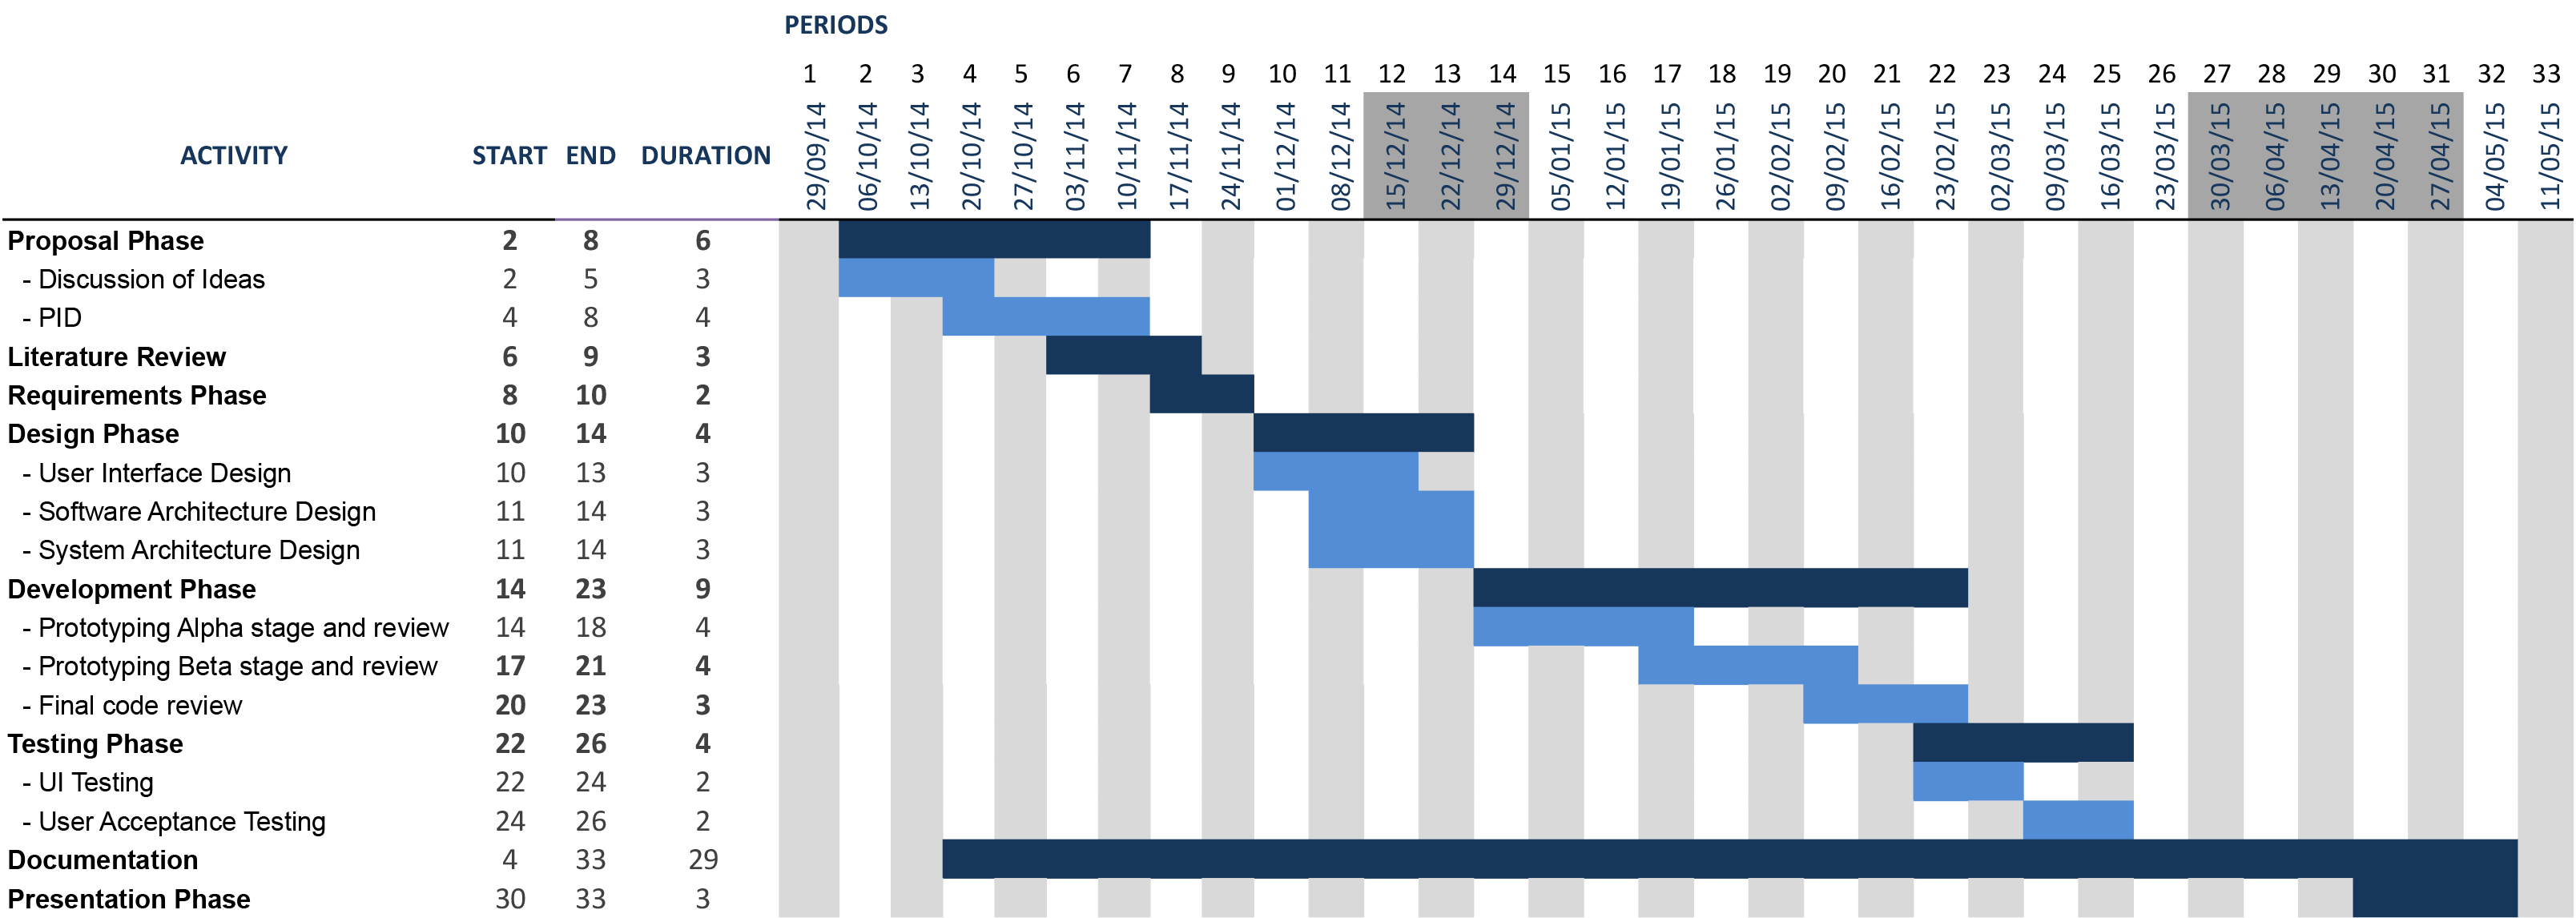
\includegraphics[width=1.28\textwidth]{./img/gantt.png}
  \end{rotate}
\end{minipage}

\clearpage
The roles are as follows:

\begin{center}
  \begin{table}[h]
  \begin{tabular}{|l|l|l|}
  \hline
  \multicolumn{1}{|c|}{\textbf{Name}} & \multicolumn{1}{c|}{\textbf{Role}} & \multicolumn{1}{c|}{\textbf{Responsibilities}}                                                                                                                                      \\ \hline
  Jay                                 & Project Manager, Developer         & \begin{tabular}[c]{@{}l@{}}Organising meetings and following the project timeline.\\ Bringing together the documentation.\\ Assisting with development when necessary.\end{tabular} \\ \hline
  Oliver                              & Technical Lead                     & \begin{tabular}[c]{@{}l@{}}Leading the technical aspects of the projects forward.\\ Managing cloud infrastructure for both documentation and code.\end{tabular}                     \\ \hline
  Simon                               & Business Development, Secretary    & \begin{tabular}[c]{@{}l@{}}Liaison with Atos.\\ Carrying the app forward according to the business model.\end{tabular}                                                              \\ \hline
  \end{tabular}
  \end{table}
\end{center}

Responsibilities will be shared as there are only three people in the team. The roles will be changing as the project progresses are some team members are stronger in different phases of the project. In the RAD Development phase for example, Oliver will be taking on the PM role as within the team he has the most expertise in terms of development and how to better organise the team. Jay will be assisting Oliver at this stage. Simon will be handing the business model of the project and liasioning with Atos when necessary. 